\section{It Is All About Apps}
\label{section_apps}
Magnolia 5.0 introduces applications of simply \emph{apps} to content
management. An \emph{app} stands for the configurable, pluggable unit which
encapsulates some certain functionality that typically operates over the data
stored in the JCR repository.
Magnolia 5.0 comes with a special framework for app management. This framework
is integrated with Magnolia CMS configuration mechanism which provides the
data required to start an app and Location Framework which triggers various
events causing app load, unload and navigation. 
There are two types of apps in Magnolia 5.0 - besides of apps of a regular type
(e.g for page editing or workspace browsing) there are special administrative so
called \emph{shell-apps}.

\subsection{Apps} An app is \emph{a tool with a very narrowly focused interface
enabling CMS users to work on one set of closely related tasks or one specific
set of data. An app does not necessarily work on a single, physical data set
(e.g. the pages of a site), but may cover multiple physical data sets required
to solve the task it covers.} \cite{maui_apps}. It is worth mentioning that in
case of Magnolia 5.0 app is not an application per se but rather a concept of a
user interface metaphor.

\subsection{App Framework}
The \emph{App Framework} is a name for Magnolia 5 functionality that manages
apps. This involves interaction with Magnolia CMS configuration mechanism:
handling the app registry and reacting on changes in app configuration.
It also controls an app life-cycle events such as starting, displaying, and
stopping an app \cite{wiki_app_framework}. Finally, the App Framework keeps the contexts of loaded apps,
maintaining their state and order.

\subsubsection{App Configuration}
The primary configuation of the apps is done by means of the
\texttt{AppDescriptor} class. \texttt{AppDescriptor} is a simple Plain Old Java
Object (POJO) that holds the meta information like the app name, label and its
icon. A descriptor also carries the name of a class that actually implements the
app and a list of \emph{sub-app} descriptors. A \emph{sub-app} is an entity that
implements the part of an app functionality. The \texttt{SubAppDescriptor} class
resembles an analogous for the app except for the fact the sub-app is a terminal
structure, so it has no child descriptors. 

In order to provide a higher level configuration mechanism for apps it is
possible to describe App descriptors in JCR inside the \emph{config} workspace.
As the Magnolia CMS web application starts up the descriptors are mapped to Java
classes by means of the Node2Bean mechanism:

\begin{figure}[H] \centering 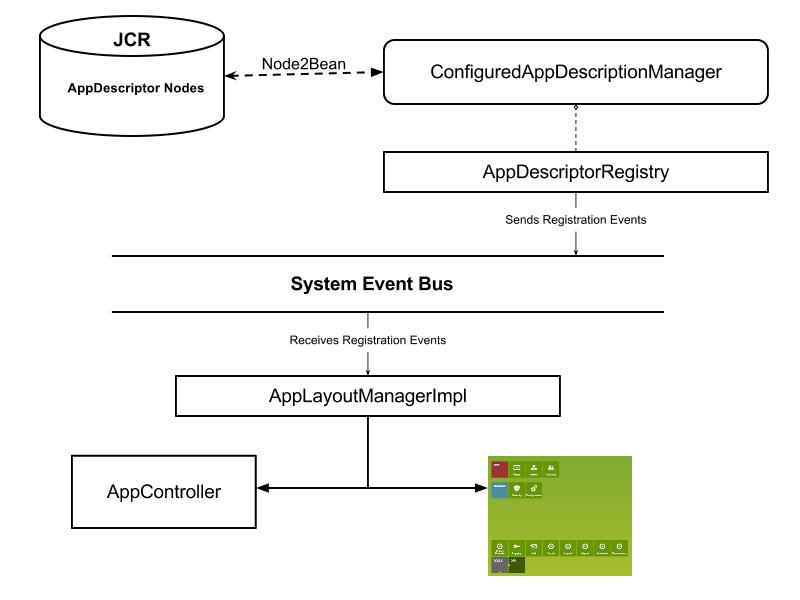
\includegraphics[width=\textwidth]{app_configuration.jpg}
	\caption{Registration of Apps.}
	\label{fig:app_registry}
\end{figure}

An instance of the \texttt{ConfiguredAppDescriptorManager} obsreves the changes 
in \emph{config} workspace and translates the JCR nodes that stand for the app descriptors to 
the objects of type \texttt{AppDescriptor}.

The scanned descriptors are then placed into the \texttt{AppDescriptorRegistry}
which fires the corresponding events for registration, deregistration or update.
The main receiver of such kind of events is an implementor of the so called
\texttt{AppLayoutManager} class. The purpose of this class is to maintain the
order of registered apps and to display them properly in the user interface (in
\emph{AppLauncher} shell-app) and to make them available to the navigation
system (the app controllers).

\begin{figure}[H] \centering 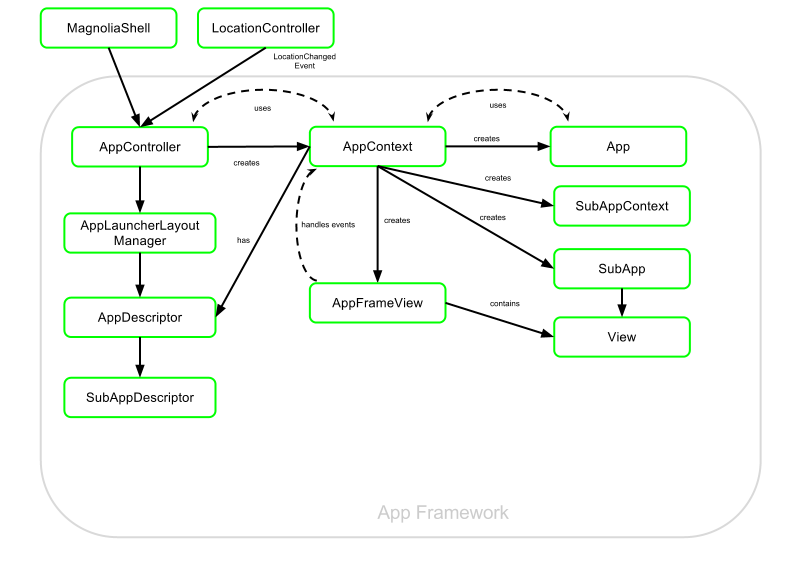
\includegraphics[width=\textwidth]{app_controller.png}
	\caption{App Context Management}
	\label{fig:app_context}
\end{figure}

\subsubsection{App Controllers and App Context.} The cornerstones of the \emph{App Framework} are the two
controller objects: \texttt{AppController} and \texttt{ShellAppController}.
These two objects play a similar role as \texttt{ActivityManager} in the original 
Places framework of GWT and apps are the analogues of \texttt{Activity}.
Controllers are subscribed to \texttt{LocationChangeEvent}'s. Based on the
incoming \texttt{Location}s either of two controllers retreives an app context.
\texttt{AppContext} is the class that holds the state of an app that is up and
running.

\begin{lstlisting}
public interface AppContext 
{
    void openSubApp(Location location);
    void start(Location location);
    void stop();
    void onLocationUpdate(Location newLocation);
    
    AppDescriptor getAppDescriptor();
    App getApp();
    
    View getView();
    String getName();    
    String mayStop();
}
\end{lstlisting}

As it is visible from the aforementioned fragment of an interface -
\texttt{AppContext} is able to react on \texttt{Location} changes. The
implementor of an interfaces typicaly conducts it by starting the app or one of
its sub-apps. An \texttt{AppContext} allocates the view component that would
host a new app (typically it is a tab-sheet component). It is also responsible
for providing all the neccessary paramteres to a newly created app or sub-app,
like dependency injector, reference to the context itself (so that the app could
indirectly communicate to the \emph{App Framework}) and location.

As the \texttt{start(\ldots)} method is called an \texttt{AppContext}
instantiates the sub-class of the \texttt{App} interface declared in the app
descriptor.

The \texttt{App} sub-class is basically a \emph{presenter} for a concrete app
implementation. We will cover the examples of app development in the
implementation chapter.

\subsection{Shell Apps.} There are three and only three shell apps that are
responsible for administration functions of the system. Those are called
\emph{AppLauncher}, \emph{Pulse} and \emph{Favorites}. \emph{AppLauncher} is a
dashboard with app icons allowing for starting apps and navigating between them.
\emph{Pulse} is an area that contains and receives the notifications and messages for a
user. Finally, \emph{Favorites} aggregates links and bookmarks allowing for better
customization of the system.